\documentclass[a4paper]{article}

\def\nbook {Differential Equations and Linear Algebra}
\def\nbookshort {DeqLA}

%%%%%%%%%%%%%%%%%%%%
% AUTHOR AND HEADER
% define \nbook
%%%%%%%%%%%%%%%%%%%%

\makeatletter
\ifx \nauthor\undefined
	\def\nauthor{David A. Lee}
\else
\fi

\author{\nbook \\ \small Gilbert Strang \\ \small Solutions by \nauthor}
\date{}

%%%%%%%%%%%%%%%%%%%%
% PACKAGES
%%%%%%%%%%%%%%%%%%%%

\usepackage{alltt} 
\usepackage{amsfonts}
\usepackage{amsmath}
\usepackage{amssymb}
\usepackage{amsthm}
\usepackage{bm}
\usepackage{booktabs}
\usepackage{caption}
\usepackage{centernot}
\usepackage{enumitem}
\usepackage{fancyhdr}
\usepackage[T1]{fontenc}
\usepackage{graphicx}
\usepackage{mathdots}
\usepackage{mathtools}
\usepackage{microtype}
\usepackage{multirow}
\usepackage{pdflscape}
\usepackage{pgfplots}
\pgfplotsset{compat=1.18}
\usepackage{siunitx}
\usepackage{slashed}
\usepackage{tabularx}
\usepackage{tikz}
\usepackage{titletoc}
\usepackage{tkz-euclide}
\usepackage[normalem]{ulem}
\usepackage{url}
\usepackage[all]{xy}
\usepackage{imakeidx}

% fonts
% use \textsf to change to Computer Modern Bright
\renewcommand{\sfdefault}{cmbr} % keeps default font Computer Modern Roman

% makeindex for table of contents
\makeindex[intoc, title=Index]
\indexsetup{othercode={\lhead{ Index }}}

% table of contents remove numbering
\usepackage{tocloft} % for coloring subsections -- note that sections have standard document hyperlink coloring, i.e. color = doc
\setcounter{secnumdepth}{0} % remove numbering
\renewcommand{\cftsubsecfont}{\hypersetup{linkcolor=subsect!90}} % subsection coloring
\renewcommand{\contentsname}{\textsf{Table of Contents}}

% pagestyle
\pagestyle{fancyplain}

% header
\lhead{	\nouppercase{\leftmark} }
\ifx \nextra \undefined
  \rhead{
    \ifnum\thepage=1
    \else
      \nbookshort \  | \nauthor
    \fi}
\else
  \rhead{
    \ifnum\thepage=1
    \else
      \nbookshort (\nextra)
    \fi}
\fi

% proof environment

\newcommand{\prooffont}{\scshape}
\usepackage{xpatch}
\tracingpatches
\xpatchcmd{\proof}{\itshape}{\prooffont}{}{}

% Python environment (for typesetting Python code)

% Default fixed font does not support bold face
\DeclareFixedFont{\ttb}{T1}{txtt}{bx}{n}{8} % for bold
\DeclareFixedFont{\ttm}{T1}{txtt}{m}{n}{8}  % for normal

% Custom colors
\usepackage{color}
\definecolor{deepblue}{rgb}{0,0,0.5}
\definecolor{deepred}{rgb}{0.6,0,0}
\definecolor{deepgreen}{rgb}{0,0.5,0}

\usepackage{listings}

% Python style for highlighting
\newcommand\pythonstyle{\lstset{
language=Python,
basicstyle=\ttm,
morekeywords={self},              % Add keywords here
keywordstyle=\ttb\color{deepblue},
emph={MyClass,__init__},          % Custom highlighting
emphstyle=\ttb\color{deepred},    % Custom highlighting style
stringstyle=\color{deepgreen},
frame=tb,                         % Any extra options here
showstringspaces=false
}}


% Python environment
\lstnewenvironment{python}[1][]
{
\pythonstyle
\lstset{#1}
}
{}

% Python for external files
\newcommand\pythonexternal[2][]{{
\pythonstyle
\lstinputlisting[#1]{#2}}}

% Python for inline
\newcommand\pythoninline[1]{{\pythonstyle\lstinline!#1!}}

%%%%%%%%%%%%%
% FUNCTIONS %
%%%%%%%%%%%%%

\DeclarePairedDelimiter\abs{\lvert}{\rvert}%
\DeclarePairedDelimiter\norm{\lVert}{\rVert}%

%%%%%%%%%%%%%%%%%%%%
% DOCUMENT GEOMETRY
%%%%%%%%%%%%%%%%%%%%

\ifx \ntrim \undefined
\else
  \usepackage{geometry}
  \geometry{
	  papersize={379pt, 699pt},
	  textwidth=345pt,
	  left=17pt,
	  top=54pt,
	  right=17pt,
  }
\fi

% maketitle statement
\title{}
\ifx \nisofficial \undefined
\let\@real@maketitle\maketitle
\renewcommand{\maketitle}{\@real@maketitle\begin{center}\begin{minipage}[c]{0.9\textwidth}\centering\footnotesize All errors, typographical and substantive, and other offenses, are entirely my own.\end{minipage}\end{center}}
\else
\fi

%%%%%%%%%%%%%%%%%%%%
% THEOREMS
%%%%%%%%%%%%%%%%%%%%

%\theoremstyle{definition}
\newtheorem*{axiom}{Axiom}
\newtheorem*{claim}{Claim}
\newtheorem*{conjecture}{Conjecture}
\newtheorem*{cor}{Corollary}
%\newtheorem*{dfn}{Definition}
\newtheorem*{eg}{Example}
\newtheorem*{ex}{Exercise}
%\newtheorem*{lemma}{Lemma}
\newtheorem*{prop}{Proposition}
%\newtheorem*{thm}{Theorem}
\newtheorem*{remark}{Remark}
\newtheorem*{warning}{Warning}

%%%%%%%%%%%%%%%%%%%%
% FORMATTING AESTHETICS
%%%%%%%%%%%%%%%%%%%%

% itemize bullets
\renewcommand{\labelitemi}{-}
\renewcommand{\labelitemii}{$\circ$}
\renewcommand{\labelenumi}{(\roman{*})}

% new page section
%\let\stdsection\section
%\renewcommand\section{\newpage\stdsection}

% new page subsection
%\let\stdsubsection\subsection
%\renewcommand\subsection{\newpage\stdsubsection}

%%%%%%%%%%%%%%%%%%%%
% \mathbb commands
%%%%%%%%%%%%%%%%%%%%

\newcommand{\C}{\mathbb{C}}
\newcommand{\N}{\mathbb{N}}
\newcommand{\Q}{\mathbb{Q}}
\newcommand{\R}{\mathbb{R}}
\newcommand{\Z}{\mathbb{Z}}

%%%%%%%%%%%%%%%%%%%%
% Complex Numbers
%%%%%%%%%%%%%%%%%%%%

\DeclareMathOperator{\Real}{Re}
\DeclareMathOperator{\Imag}{Im}

%%%%%%%%%%%%%%%%%%%%
% Probability Operators
%%%%%%%%%%%%%%%%%%%%

\DeclareMathOperator{\Bernoulli}{Bernoulli}
\DeclareMathOperator{\betaD}{Beta}
\DeclareMathOperator{\bias}{\textsf{bias}}
\DeclareMathOperator{\binomial}{Binomial}
\DeclareMathOperator{\corr}{Corr}
\DeclareMathOperator{\cov}{\textsf{Cov}}
\DeclareMathOperator{\Exp}{Exp}
\DeclareMathOperator{\gammaD}{Gamma}
\DeclareMathOperator{\mse}{\textsf{MSE}}
\DeclareMathOperator{\multinomial}{Multinomial}
\DeclareMathOperator{\Poisson}{Poisson}
\DeclareMathOperator{\sd}{sd}
\DeclareMathOperator{\se}{\textsf{se}}
\DeclareMathOperator{\Uniform}{Uniform}
\newcommand{\Prob}{\mathbb{P}}
\newcommand{\var}{\mathbb{V}}
\newcommand{\E}{\mathbb{E}}

%%%%%%%%%%%%%%%%%%%%
% TCOLORBOX CODE FROM SeniorMars
%%%%%%%%%%%%%%%%%%%%

%\usepackage[varbb]{newpxmath} changes math font to newpxmath
\usepackage{xfrac}
\usepackage[makeroom]{cancel}
\usepackage{mathtools}
\usepackage{bookmark}
\usepackage{enumitem}
\usepackage{hyperref}
\usepackage{theoremref}
\hypersetup{
	pdftitle={Assignment},
	colorlinks=true, linkcolor=doc!90,
	bookmarksnumbered=true,
	bookmarksopen=true
}
\usepackage[most,many,breakable]{tcolorbox}
\usepackage{xcolor}
\usepackage{varwidth}
\usepackage{varwidth}
\usepackage{etoolbox}
%\usepackage{authblk}
\usepackage{nameref}
\usepackage{multicol,array}
\usepackage{tikz-cd}
\usepackage[ruled,vlined,linesnumbered]{algorithm2e}
\usepackage{comment} % enables the use of multi-line comments (\ifx \fi)
\usepackage{import}
\usepackage{xifthen}
\usepackage{pdfpages}
\usepackage{transparent}

\newcommand\mycommfont[1]{\footnotesize\ttfamily\textcolor{blue}{#1}}
\SetCommentSty{mycommfont}
\newcommand{\incfig}[1]{%
    \def\svgwidth{\columnwidth}
    \import{./figures/}{#1.pdf_tex}
}

\usepackage{tikzsymbols}

% colors -- change them as you may!

\definecolor{myg}{RGB}{56, 140, 70}
\definecolor{myb}{RGB}{45, 111, 177}
\definecolor{myr}{RGB}{199, 68, 64}
\definecolor{mytheorembg}{HTML}{F2F2F9}
\definecolor{mytheoremfr}{HTML}{00007B}
\definecolor{mylenmabg}{HTML}{FFFAF8}
\definecolor{mylenmafr}{HTML}{983b0f}
\definecolor{mypropbg}{HTML}{f2fbfc}
\definecolor{mypropfr}{HTML}{191971}
\definecolor{myexamplebg}{HTML}{F2FBF8}
\definecolor{myexamplefr}{HTML}{88D6D1}
\definecolor{myexampleti}{HTML}{2A7F7F}
\definecolor{mydefinitbg}{HTML}{E5E5FF}
\definecolor{mydefinitfr}{HTML}{3F3FA3}
\definecolor{notesgreen}{RGB}{0,162,0}
\definecolor{myp}{RGB}{197, 92, 212}
\definecolor{mygr}{HTML}{880808}
\definecolor{myred}{RGB}{127,0,0}
\definecolor{myyellow}{RGB}{169,121,69}
\definecolor{myexercisebg}{HTML}{F2FBF8}
\definecolor{myexercisefg}{HTML}{88D6D1}
\definecolor{doc}{RGB}{0,0,255}
\definecolor{subsect}{RGB}{255,0,0}
\definecolor{question}{HTML}{3FB69E}

%================================
% THEOREM BOX
%================================

%\providecommand\theoremnumber{}
\tcbuselibrary{theorems,skins,hooks}
\newtcbtheorem{Theorem}{Theorem}
{%
	enhanced,
	breakable,
	colback = mytheorembg,
	frame hidden,
	boxrule = 0sp,
	borderline west = {2pt}{0pt}{mytheoremfr},
	sharp corners,
	detach title,
	before upper = \tcbtitle\par\smallskip,
	coltitle = mytheoremfr,
	fonttitle = \bfseries\sffamily,
	description font = \mdseries,
	separator sign none,
	segmentation style={solid, mytheoremfr},
}
{th}


%================================
% Question BOX
%================================

\makeatletter
\newtcbtheorem{question}{Question}{enhanced,
	breakable,
	colback=white,
	colframe=question,
	attach boxed title to top left={yshift*=-\tcboxedtitleheight},
	fonttitle=\bfseries\sffamily,
	title={#2},
	boxed title size=title,
	boxed title style={%
			sharp corners,
			rounded corners=northwest,
			colback=tcbcolframe,
			boxrule=0pt,
		},
	underlay boxed title={%
			\path[fill=tcbcolframe] (title.south west)--(title.south east)
			to[out=0, in=180] ([xshift=5mm]title.east)--
			(title.center-|frame.east)
			[rounded corners=\kvtcb@arc] |-
			(frame.north) -| cycle;
		},
	#1
}{def}
\makeatother

%================================
% PROPERTIES BOX
%================================

\tcbuselibrary{theorems,skins,hooks}
\newtcbtheorem{Property}{Property}
{%
	enhanced,
	breakable,
	colback = mytheorembg,
	frame hidden,
	boxrule = 0sp,
	borderline west = {2pt}{0pt}{mytheoremfr},
	sharp corners,
	detach title,
	before upper = \tcbtitle\par\smallskip,
	coltitle = mytheoremfr,
	fonttitle = \bfseries\sffamily,
	description font = \mdseries,
	separator sign none,
	segmentation style={solid, mytheoremfr},
}
{th}

%================================
% LEMMA
%================================

\tcbuselibrary{theorems,skins,hooks}
\newtcbtheorem[number within=section]{Lemma}{Lemma}
{%
	enhanced,
	breakable,
	colback = mylenmabg,
	frame hidden,
	boxrule = 0sp,
	borderline west = {2pt}{0pt}{mylenmafr},
	sharp corners,
	detach title,
	before upper = \tcbtitle\par\smallskip,
	coltitle = mylenmafr,
	fonttitle = \bfseries\sffamily,
	description font = \mdseries,
	separator sign none,
	segmentation style={solid, mylenmafr},
}
{th}


% Commands for special boxes
\newcommand{\thm}[2]{\begin{Theorem*}{#1}{}#2\end{Theorem*}}
\newcommand{\qs}[2]{\begin{question*}{#1}{}#2\end{question*}}
\newcommand{\prp}[2]{\begin{Property*}{#1}{}#2\end{Property*}}
\newcommand{\lemma}[2]{\begin{Lemma*}{#1}{}#2\end{Lemma*}}


\begin{document}
\maketitle

\newpage
\tableofcontents

\newpage
\section{\textsf{2 - Second Order Equations}}

\subsection{\textsf{2.1 - Second Derivatives in Science and Engineering}}

% QUESTION 1
\qs{2.1.1}{Find a cosine and a sine that solve \(d^{2}y / dt^{2} = -9y\). This is a second order equation so we expect \textit{two constants} \(C\) and \(D\) (from integrating twice):
\[
	\textbf{Simple harmonic motion} \quad y \!\left( t \right) = C \cos\left( \omega t \right) + D \sin\left( \omega t \right) 
\]

What is \(\omega\)? If the system starts from rest (this means \(dy/dt = 0\) at \(t = 0\)), which constant \(C\) or \(D\) will be zero?
}

Differentiating \(y \!\left( t \right) \) twice, we get a \(\omega^{2}\) term. Making the necessary substitutions, we can see that \(\omega^{2} = 9\), implying \(\omega = 3\). Thus we have \(y = \sin\left( 3t \right)\) and \(y = \cos\left( 3t \right)\). The constants \(C\) and \(D\) are determined by the initial conditions. Assuming the system starts at rest, we must have

\[
	\frac{d y}{d t} = - 3C \sin\left( 3t \right) + 3D \cos\left( 3t \right) = 0
\]
which implies that \(dy / dt_{t = 0} = 3D = 0\), thus \(D = 0\).

\vspace{12pt}

% QUESTION 2
\qs{2.1.2}{In Problem 1, which \(C\) and \(D\) will give the starting values \(y \!\left( 0 \right) = 0\) and \(y' \!\left( 0 \right) = 1\)?}

We have \(y \!\left( 0 \right) = C = 0\) and \(y' \!\left( 0 \right) = 3D = 1\), or \(D = 1/3\).

\newpage

% QUESTION 3
\qs{2.1.3}{Draw Figure 2.3 to show simple harmonic motion \(y = A \cos\left( \omega t - \alpha  \right)\) with phases \(\alpha = \pi / 3\) and \(\alpha = -\pi /2\).}

\begin{center}
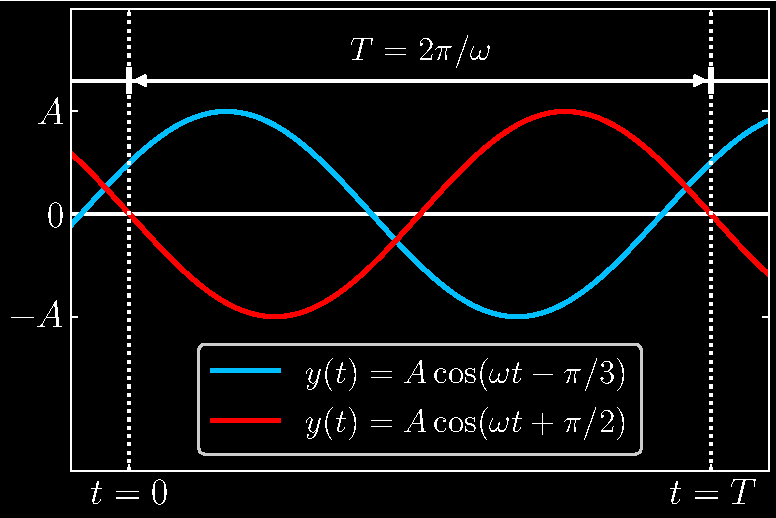
\includegraphics[width=1.0\textwidth]{../chap2/sec2.1/chap2sec2.1ex3.eps}
\end{center}

% QUESTION 4
\qs{2.1.4}{Suppose the circle in Figure 2.4 has radius 3 and circular frequency \(f = 60\) Hertz. If the moving point starts at the angle \(-45^{\circ}\), find its \(x\)-coordinate \(A \cos\left( \omega t - \alpha  \right)\). The phase lag is \(\alpha = 45^{\circ}\). When does the point first hit the \(x\)-axis?}

The circular motion of the point is expressed by the sinusoidal
\[
	3 \cos\left( 120 \pi t - \frac{\pi }{4} \right)
\]
Note that since the frequency is \(f = 60\) Hertz, the angular frequency is \(2 \pi \cdot 60 = 120 \pi \) radians s\(^{-1}\). The point hits the \(x\)-axis when the argument of the cosine is zero, namely at
\[
	120 \pi t - \frac{\pi }{4} = 0 \quad \implies \quad t = \frac{1}{480} \text{s}
\]

% QUESTION 5
\qs{2.1.5}{If you drive at 60 miles per hour on a circular track with radius \(R = 3\) miles, what is the time \(T\) for one complete circuit? Your circular frequency is \(f = \) \underline{\qquad} and your angular frequency is \(\omega = \) \underline{\qquad} (with what units?). The period is \(T\).}

Using dimensional analysis, the period is
\[
	T = \frac{1 \text{ hr}}{60 \text{ mi}} \!\left( 3 \text{ mi} \right) = \frac{1}{20} \text{ hr}
\]
The circular frequency is
\[
	f = \frac{60 \text{ mi}}{\text{ hr}} \frac{1 \text{ hr}}{3600 \text{ s}} \frac{1 \text{ cycle}}{3 \text{ mi}} = \frac{1}{180} \text{ s}^{-1}
\]
with angular frequency
\[
	\omega = 2 \pi f = \frac{\pi }{90} \text{ rad s}^{-1}
\]

% QUESTION 6
\qs{2.1.6}{The total energy \(E\) in the oscillating spring-mass system is
\begin{alignat*}{2}
	E & = \textbf{kinetic} \text{ energy in mass} + \textbf{potential} \text{ energy in spring} \\
	  & = \frac{m}{2} \!\left( \frac{d y}{d t}  \right)^{2} + \frac{k}{2}y^{2}
\end{alignat*}
Compute \(E\) when \(y = C \cos\left( \omega t \right) + D \sin\left( \omega t \right)\). The energy is constant!}

Given \(y \!\left( t \right) \), we have first time-derivative
\[
	\frac{d y}{d t} = - \omega C \sin\left( \omega t \right) + \omega D \cos\left( \omega t \right)
\]
squaring gives us
\[
	\!\left( \frac{d y}{d t}  \right)^{2} = \omega^{2} \!\left( C^{2} \sin^{2}\left( \omega t \right) - 2 CD \sin\left( \omega t \right) \cos\left( \omega t \right) + D^{2}\cos^{2}\left( \omega t \right) \right)
\]
Lastly, the \(y^{2}\) term is
\[
	y^{2} = C^{2} \cos^{2}\left( \omega t \right) + 2CD \sin\left( \omega t \right)\cos\left( \omega t \right) + D^{2}\sin^{2}\left( \omega t \right)
\]
Combining our ingredients, with \(\omega = \sqrt{k / m}\), observe that energy \(E\) reduces to a constant:
\begin{alignat*}{2}
	E & = \frac{m}{2} \!\left( \frac{d y}{d t}  \right)^{2} + \frac{k}{2} y^{2} \\
	  & = \frac{m}{2} \!\left( \frac{k}{m} \right) \!\left( C^{2}\sin^{2}\left( \omega t \right) - 2CD \sin\left( \omega t \right) \cos\left( \omega t \right) + D^{2} \cos^{2}\left( \omega t \right)\right)  \\ 
	  & \qquad + \frac{k}{2} \!\left( C^{2} \cos^{2}\left( \omega t \right) + 2CD \sin\left( \omega t \right)\cos\left( \omega t \right) + D^{2}\sin^{2}\left( \omega t \right) \right) \\
	  & = C^{2} + D^{2}
\end{alignat*}

\newpage

% QUESTION 7
\qs{2.1.7}{Another way to show that the total energy \(E\) is constant:

Multiply \(\bm{my'' + ky = 0}\) by \(\bm{y'}\). Then integrate \(my'y''\) and \(kyy'\).}

Take the first term and integrate:
\[
	m \int y'y'' \, dt
\]
By integration by parts, let
\[
	u = \frac{d y}{d t}, \quad \frac{d u}{d t} = \frac{d^{2}y}{d t^{2}} \quad \implies \quad du = \frac{d^{2}y}{d t^{2}} dt 
\]
Then we can rewrite the first term as
\[
	m \int u \, du = \frac{m}{2}u^{2} + C = \frac{m}{2} \!\left( y' \right)^{2} + C 
\]
as for the second term:
\[
	k \int yy' \, dt = k \int y \frac{d y}{d t}  \, dt = k \int y \, dy = \frac{k}{2}y^{2} + C 
\]
Summing the two pieces (sans the constants) restores the original energy function:
\[
	E = \frac{m}{2} \!\left( \frac{d y}{d t}  \right)^{2} + \frac{k}{2}y^{2}
\]
and since the derivative of a constant is zero, it must be the case that \(E\) is a constant.

\vspace{12pt}

% QUESTION 8
\qs{2.1.8}{A \textbf{forced oscillation} has another term in the equation and \(A \cos\left( \omega t \right)\) in the solution:
\[
	\frac{d^{2}y}{dt^{2}} + 4y = F \cos\left( \omega t \right) \quad \text{has} \quad y = C \cos\left( 2 t \right) + D \sin\left( 2 t \right) + A \cos\left( \omega t \right)
\]
\begin{enumerate}[label=(\alph*)]
	\item Substitute \(y\) into the equation to see how \(C\) and \(D\) disappear (they give \(y_{n}\). Find the forced amplitude \(A\) in the particular solution \(y_{p} = A \cos\left( \omega t \right)\).
	\item In case \(\omega = 2\) (forcing frequency \(=\) natural frequency), what answer does your formula give for \(A\)? The solution formula for \(y\) breaks down in this case.
\end{enumerate}}

The second time-derivative is
\[
	\frac{d^{2}y}{dt^{2}} = -4C \cos\left( 2t \right) - 4D \sin\left( 2t \right) - \omega^{2}A \cos\left( \omega t \right)
\]
\begin{enumerate}[label=(\alph*)]
	\item We have
		\[
			\frac{d^{2}y}{dt^{2}} + 4y = \!\left( 4 - \omega^{2} \right) A \cos\left( \omega t \right) = F \cos\left( \omega t \right)
		\]
	implying \(A = \dfrac{F}{4 - \omega^{2}}\).
	\item When \(\omega = 2\), \(A\) is undefined. 
\end{enumerate}

% QUESTION 9
\qs{2.1.9}{Following Problem 8, write down the complete solution \(y_{n} + y_{p}\) to the equation
\[
	m \frac{d^{2}y}{dt^{2}} + ky = F \cos\left( \omega t \right) \quad \text{with} \quad \omega \neq \omega_{n} = \sqrt{k / m} \quad \text{(no resonance)}
\]
The answer \(y\) has free constants \(C\) and \(D\) to match \(y \!\left( 0 \right) \) and \(y'\!\left( 0 \right) \) (\(A\) \textit{is fixed} by \(F\).}

Per Problem 8, we have solution
\[
	y = \underbrace{C \cos\left( \sqrt{\frac{k}{m}} t \right) + D \sin\left( \sqrt{\frac{k}{m}} t \right)}_{y_{n}} + \underbrace{\frac{F}{k - m \omega^{2}} \cos\left( \omega t \right)}_{y_{p}}
\]

All this involves is dividing the equation through by \(m\), understanding that the angular frequency of the sinusoidals in the null solution is the square root of \(k / m\), and making the changes to our formula for \(A\) accordingly.

\vspace{12pt}

% QUESTION 10
\qs{2.1.10}{Suppose Newton's Law \(F = ma\) has the force \(F\) in the \textit{same} direction as \(a\):
\[
	my'' = + ky \quad \text{including} \quad y'' = 4y
\]
Find two possible choices of \(s\) in the exponential solutions \(y = e^{st}\). The solution is not sinusoidal and \(s\) is real and the oscillations are gone. Now \(y\) is unstable.}

Substituting in \(y\), we find
\[
	ms^{2}e^{st} = ke^{st}
\]
This forces
\[
	s = \pm \sqrt{\frac{k}{m}}
\]
\newpage

% QUESTION 11
\qs{2.1.11}{Here is a \textit{fourth} order equation: \(d^{4}y / dt^{4} = 16y\). Find \textit{four} values of \(s\) that give exponential solutions \(y = e^{st}\). You could expect four initial conditions on \(y\): \(y \!\left( 0 \right) \) is given along with what three other conditions?}

Equivalently, we find the four complex roots of \(16\):
\[
	s^{4} = 16
\]
which are \(s = \pm 2, \pm 2i\).

\vspace{12pt}

% QUESTION 12
\qs{2.1.12}{To find a particular solution to \(y'' + 9y = e^{ct}\), I would look for a multiple \(y_{p}\!\left( t \right) = Ye^{ct}\) of the forcing function. What is that number \(Y\)? When does your formula give \(Y = \infty\)? (Resonance needs a new formula for \(Y\).)}

Let \(y_{p} = Ye^{ct}\). Substituting, we find
\[
	Yc^{2} e^{ct} + 9Ye^{ct} = e^{ct}
\]
Solving for \(Y\) yields \(Y = \dfrac{1}{c^{2} + 9}\). When \(c \rightarrow \pm3\), we have resonance, and \(Y \rightarrow \infty\).

\vspace{12pt}

% QUESTION 13
\qs{2.1.13}{In a particular solution \(y = Ae^{i \omega t}\) to \(y'' + 9y = e^{i \omega t}\), what is the amplitude \(A\)? The formula blows up when the forcing frequency \(\omega =\) what natural frequency?}

Substituting, we derive
\[
	-\omega^{2}A e^{i \omega t} + 9A e^{i \omega t} = e^{i \omega t}
\]
which gives us \(A = \dfrac{1}{9 - \omega^{2}}\). Resonance is when \(\omega = 3\).

\vspace{12pt}

\newpage
% QUESTION 14
\qs{2.1.14}{Equation (10) says that the tangent of the phase angle is \(\tan\left( \alpha  \right) = y' \!\left( 0 \right) / \omega y \!\left( 0 \right) \). First, check that \(\tan\left( \alpha  \right)\) is dimensionless when \(y\) is in meters and time is in seconds. Next, if that ratio is \(\tan\left( \alpha  \right) = 1\), should you choose \(\alpha = \pi / 4\) or \(\alpha = 5 \pi / 4\)? Answer:
\[
	\text{Separately you want } R \cos \left( \alpha  \right) = y \!\left( 0 \right)  \text{ and } R \sin \left( \alpha  \right) = y' \!\left( 0 \right) / \omega 
\]
If those right hand sides are positive, choose the angle \(\alpha \) between \(0\) and \(\pi / 2\). 

If those right hand sides are negative, add \(\pi \) and choose \(\alpha = 5 \pi / 4\).

\vspace{12pt}

\textit{Question}: If \(y \!\left( 0 \right) > 0\) and \(y' \!\left( 0 \right) < 0\), does \(\alpha \) fall between \(\pi / 2\) and \(\pi \) or between \(3 \pi / 2\) and \(2 \pi \)? If you plot the vector from \( \!\left( 0, 0 \right) \) to \(\!\left( y \!\left( 0 \right) , y' \!\left( 0 \right) / \omega  \right) \), its angle is \(\alpha \).}

As \(y \!\left( 0 \right) > 0\) and \(y'\!\left( 0 \right) < 0\) requires positive cosine and negative sine, \(\alpha \) falls between \(3 \pi / 2\) and \(2 \pi \).

\vspace{12pt}

% QUESTION 15
\qs{2.1.15}{Find a point on the sine curve in Figure 2.1 where \(y > 0\) but \(v = y' < 0\) and also \(a = y'' < 0\). The curve is sloping down and bending down.

\vspace{12pt}

Find a point where \(y < 0\) but \(y' > 0\) and \(y'' > 0\). The point is below the \(x\)-axis but the curve is sloping \underline{\qquad} and bending \underline{\qquad}.}

One area corresponding to the first set of conditions is \(\pi / 2 < t < \pi \). As for the second, we have \(3 \pi / 2 < t < 2 \pi \).

\vspace{12pt}

% QUESTION 16
\qs{2.1.16}{
\begin{enumerate}[label=(\alph*)]
	\item Solve \(y'' + 100y = 0\) starting from \(y \!\left( 0 \right) = 1\) and \(y' \!\left( 0 \right) = 10\). (\( \textbf{This is } \bm{y_{n}} \).)
	\item Solve \(y'' + 100y = \cos\left( \omega t \right)\) with \(y \!\left( 0 \right) = 0\) and \(y' \!\left( 0 \right) = 0\). (\( \textbf{This can be }\bm{y_{p}} \).)
\end{enumerate}}

\begin{enumerate}[label=(\alph*)]
	\item Let \(y = c_{1} \cos\left( 10 t \right) + c_{2} \sin\left( 10 t \right)\). Then \(y \!\left( 0 \right) = c_{1} = 1\) and \(y' \!\left( 0 \right) = 10 c_{2} = 10\) implies \(c_{2} = 1\). Then the null solution is
	\[
		y_{n} = \cos\left( 10 t \right) + \sin\left( 10 t \right)
	\]
\item Let \(y_{p} = R \cos\left( \omega t \right)\). Substitute to find
	\[
		-\omega^{2} R \cos\left( \omega t \right) + 100 R \cos\left( \omega t \right) = \cos\left( \omega t \right)
	\]
	Isolate \(R\) to derive
	\[
		R = \frac{1}{100 - \omega^{2}}
	\]
	The solution to this set of initial conditions requires \(y \!\left( 0 \right) = 0 \) and \(y' \!\left( 0 \right) = 0\). Begin with
	\[
		y \!\left( t \right) = c_{1} \cos\left( 10 t \right) + c_{2} \sin\left( 10 t \right) + \frac{1}{100 - \omega^{2}} \cos\left( \omega t \right)	
	\]
	From the first condition, we have \(c_{1} = -\dfrac{1}{100 - \omega^{2}}\). From the second, we have \(c_{2} = 0\). The full solution is
	\[
		y \!\left( t \right) = \frac{1}{100 - \omega^{2}} \!\left( \cos\left( \omega t \right) - \cos\left( 10t \right) \right) 
	\]
\end{enumerate}

% QUESTION 17
\qs{2.1.17}{Find a particular solution \(y_{p} = R \cos\left( \omega t - \alpha  \right)\) to \(y'' + 100y = \cos\left( \omega t \right) - \sin\left( \omega t \right)\).}

Substituting \(y_{p}\) gives us

\begin{alignat*}{2}
	& -\omega^{2} R \cos\left( \omega t - \alpha  \right) + 100 R \cos\left( \omega t - \alpha  \right) \\
		 & \qquad = \!\left( 100R - \omega^{2}R \right) \!\left[ \cos\left( \omega t \right)\cos\left( \alpha  \right) + \sin\left( \omega t \right)\sin\left( \alpha  \right) \right]  \\
\end{alignat*}

This implies that
\begin{alignat*}{2}
	R \cos\left( \alpha  \right) \!\left( 100 - \omega^{2} \right) & = 1 \\
	R \sin\left( \alpha  \right) \!\left( 100 - \omega^{2} \right) & = -1 \\ 
\end{alignat*}
enabling us to conclude that \(\alpha = 7 \pi / 4\), and amplitude
\[
	R = \frac{\sqrt{2}}{100 - \omega^{2}}
\]
Ergo, the particular solution is
\[
	y_{p} = \frac{\sqrt{2}}{100 - \omega^{2}} \cos\left( \omega t - \frac{7 \pi }{4} \right)
\]

% QUESTION 18
\qs{2.1.18}{Simple harmonic motion also comes from a linear pendulum (like a grandfather clock). At time \(t\), the height is \(A \cos\left( \omega t \right)\). What is the frequency \(\omega \) if the pendulum comes back to the start after 1 second? The period does not depend on the amplitude (a large clock or a small metronome or the movement in a watch can all have \(T = 1\)).}

The angular frequency is \(2 \pi \cdot f = 2 \pi \) radians s\(^{-1}\).

\vspace{12pt}

% QUESTION 19
\qs{2.1.19}{If the phase lag is \(\alpha \), what is the time lag in graphing \(\cos\left( \omega t - \alpha \right)\)?}

Put differently, we want to find the value of \(t'\) such that we are able to restore \(\omega t\) as the cosine's argument. If we have
\[
	t' = t + \alpha / \omega 
\]
then we get
\[
	\cos\left( \omega t' - \alpha  \right) = \cos\left( \omega \!\left( t + \alpha / \omega  \right) - \alpha  \right) = \cos\left( \omega t \right)
\]
Thus the time lag term is \(\alpha / \omega \).

\vspace{12pt}

% QUESTION 20
\qs{2.1.20}{What is the response \(y \!\left( t \right) \) to a delayed impulse if \(my'' + ky = \delta \!\left( t - T \right) \)?}

The full solution will be a factor of the step function, given by:
\[
	y \!\left( t \right) = \int^{t - T}_{0} \frac{\sin\left( \omega_{n} \!\left( t - T - s \right)  \right)}{m \omega_{n}} \delta \!\left( s \right)  \, ds = \frac{\sin\left( \omega_{n} \!\left( t - T \right)  \right)}{m \omega_{n}} H \!\left( t - T \right) 
\]
Intuitively, when \(t \le T\), the right-hand side vanishes. No impulse is imparted, and thus there is no response. But when we are at time \(t \ge T\) -- after the threshold -- the response kicks in.
\vspace{12pt}

% QUESTION 21
\qs{2.1.21}{(Good challenge) Show that \(\displaystyle{y = \int^{t}_{0} g \!\left( t - s \right) f \!\left( s \right)  \, ds }\) has \(my'' + ky = f \!\left( t \right) \).

\begin{enumerate}[label=\arabic*.]
	\item Why is \(\displaystyle{y' = \int^{t}_{0} g'\!\left( t - s \right) f \!\left( s \right)  \, ds + g \!\left( 0 \right) f \!\left( t \right)  }\)? Notice the two \(t\)'s in \(y\).
	\item Using \(g \!\left( 0 \right) = 0\), explain why \(\displaystyle{y'' = \int^{t}_{0} g''\!\left( t - s \right) f \!\left( s \right)  \, ds + g'\!\left( 0 \right) f \!\left( t \right)  }\).
	\item Now use \(g'\!\left( 0 \right) = 1 / m\) and \(mg'' + kg = 0\) to confirm \(my'' + ky = f \!\left( t \right) \).
\end{enumerate}}

Use the Leibniz integral rule:
\[
	\frac{d }{d t} \!\left( \int^{t}_{0} g \!\left( t - s \right) f \!\left( s \right)  \, ds \right) = g\!\left( 0 \right) f \!\left( t \right) + \int^{t}_{0} \frac{\partial }{\partial t} g \!\left( t - s \right) f \!\left( s \right)  \, ds 
\]

\begin{enumerate}[label=(\arabic*)]
	\item By above, applying the partial derivative inside the second term yields the desired result.
	\item One more application of the Leibniz rule gives us
	\[
		y'' = \int^{t}_{0} g''\!\left( t - s \right) f \!\left( s \right)  \, ds + g \!\left( 0 \right) f'\!\left( t \right) + g'\!\left( 0 \right) f \!\left( t \right) 
	\]
	With the premise \(g \!\left( 0 \right) = 0\), the second term vanishes and gives us the expected result.
	\item Derive
	\[
		my'' + ky = \int^{t}_{0} \!\left[ mg''\!\left( t - s \right) + kg \!\left( t - s \right)  \right] f \!\left( s \right)  \, ds + f \!\left( t \right) = f \!\left( t \right)   \\
	\]
	where the last equality follows by appealing to the nullity of \(g \!\left( t \right) \).
\end{enumerate}

% QUESTION 22
\qs{2.1.22}{With \(f = 1\) (direct current has \(\omega = 0\)) verify that \(my'' + ky = 1\) for this \(y\):
\[
	\textbf{Step response}
\]
\[
	y \!\left( t \right) = \int^{t}_{0} \frac{\sin\left( \omega_{n} \!\left( t - s \right)  \right)}{m \omega_{n}} \cdot 1 \, ds = y_{p} + y_{n} = \pmb{\frac{1}{k} - \frac{1}{k} \cos\left( \omega_{n}t \right)}
\]}

We have second derivative
\[
	y''\!\left( t \right) = \frac{\omega_{n}^{2}}{k}\cos\left( \omega_{n}t \right)	
\]
Since \(\omega_{n} = \sqrt{k / m}\), \(my''\!\left( t \right) = \cos\left( \omega_{n}t \right)\). Ergo, we have
\[
	my'' + ky = \cos\left( \omega_{n}t \right) + k \!\left[ \frac{1}{k} - \frac{1}{k}\cos\left( \omega_{n}t \right) \right] = 1
\]

% QUESTION 23
\qs{2.1.23}{(Recommended) For the equation \(d^{2}y / dt^{2} = 0\) find the null solution. Then for \(d^{2}g / dt^{2} = \delta \!\left( t \right) \) find the fundamental solution (start the null solution with \(g \!\left( 0 \right) = 0\) and \(g'\!\left( 0 \right) = 1\)). For \(y'' = f \!\left( t \right) \) find the particular solution using formula (16).}

Integrating twice, the null solution is
\[
	y \!\left( t \right) = C_{1} t + C_{2}
\]
To find the fundamental solution \(g \!\left( t \right) \), imposing the initial conditions \(g \!\left( 0 \right) = 0\) and \(g'\!\left( 0 \right) = 1\) forces \(C_{1} = 1\) and \(C_{2} = 0\), thus
\[
	g \!\left( t \right) = t
\]
Lastly, if \(y'' = f \!\left( t \right) \), then
\[
	y_{p}\!\left( t \right) = \int^{t}_{0} \!\left( t - s \right) f \!\left( s \right)  \, ds 
\]
% QUESTION 24
\qs{2.1.24}{For the equation \(d^{2}y/ dt^{2} = e^{i \omega t}\) find a particular solution \(y = Y \!\left( \omega  \right) e^{i \omega t}\). Then \(Y \!\left( \omega  \right) \) is the frequency response. Note the ``resonance'' when \(\omega = 0\) with the null solution \(y_{n} = 1\).}

One particular solution is
\[
	y \!\left( t \right) = -\frac{e^{i \omega t}}{\omega^{2}}
\]
meaning that \(Y \!\left( \omega  \right) = - 1 / \omega^{2}\). When \(\omega = 0\), we have resonance, and this particular solution breaks down.

\vspace{12pt}

% QUESTION 25
\qs{2.1.25}{Find a particular solution \(Ye^{i \omega t}\) to \(my'' - ky = e^{i \omega t}\). The equation has \(-ky\) instead of \(ky\). What is the frequency response \(Y \!\left( \omega  \right) \)? For which \(\omega \) is \(Y\) infinite?}

We have
\[
	\frac{d^{2} }{d t^{2}} \!\left( Y e^{i \omega t} \right) = - Y \omega^{2} e^{i \omega t}
\]
Substituting and canceling the \(e^{i \omega t}\) terms, we get
\[
	-mY \omega^{2} - kY = 1
\]
Implying
\[
	Y \!\left( \omega  \right) = -\frac{1}{m \omega^{2} + k}
\]
If we have
\[
	\omega = i \sqrt{\frac{k}{m}}
\]
then \(Y \!\left( \omega  \right) \) diverges to infinity -- meaning all real frequencies will not lead to this!

\newpage

\subsection{\textsf{2.2 - Key Facts About Complex Numbers}}

% QUESTION 1
\qs{2.2.1}{Mark the numbers \(s_{1} = 2 + i\) and \(s_{2} = 1 - 2i\) as points in the complex plane. (The plane has a real axis and an imaginary axis.) Then mark the sum \(s_{1} + s_{2}\) and the difference \(s_{1} - s_{2}\).}

\end{document}
